\chapter{System Presentation}
\label{sub:page}
The project group page is the virtual meeting place described in \secref{sec:projectgroup}.
We decided to implement the room merely as a container for blocks. 
Alternatively the functionality could be an integrated part of the page, but using blocks gives more flexibility to the users allowing them manage the layout of their own project group room. 
A screenshot of a project group room can be seen in \figref{fig:projectgroupnoedit}. 
In this project group room the blocks of the standard layout are seen.
\begin{figure}[h]
	\centering
		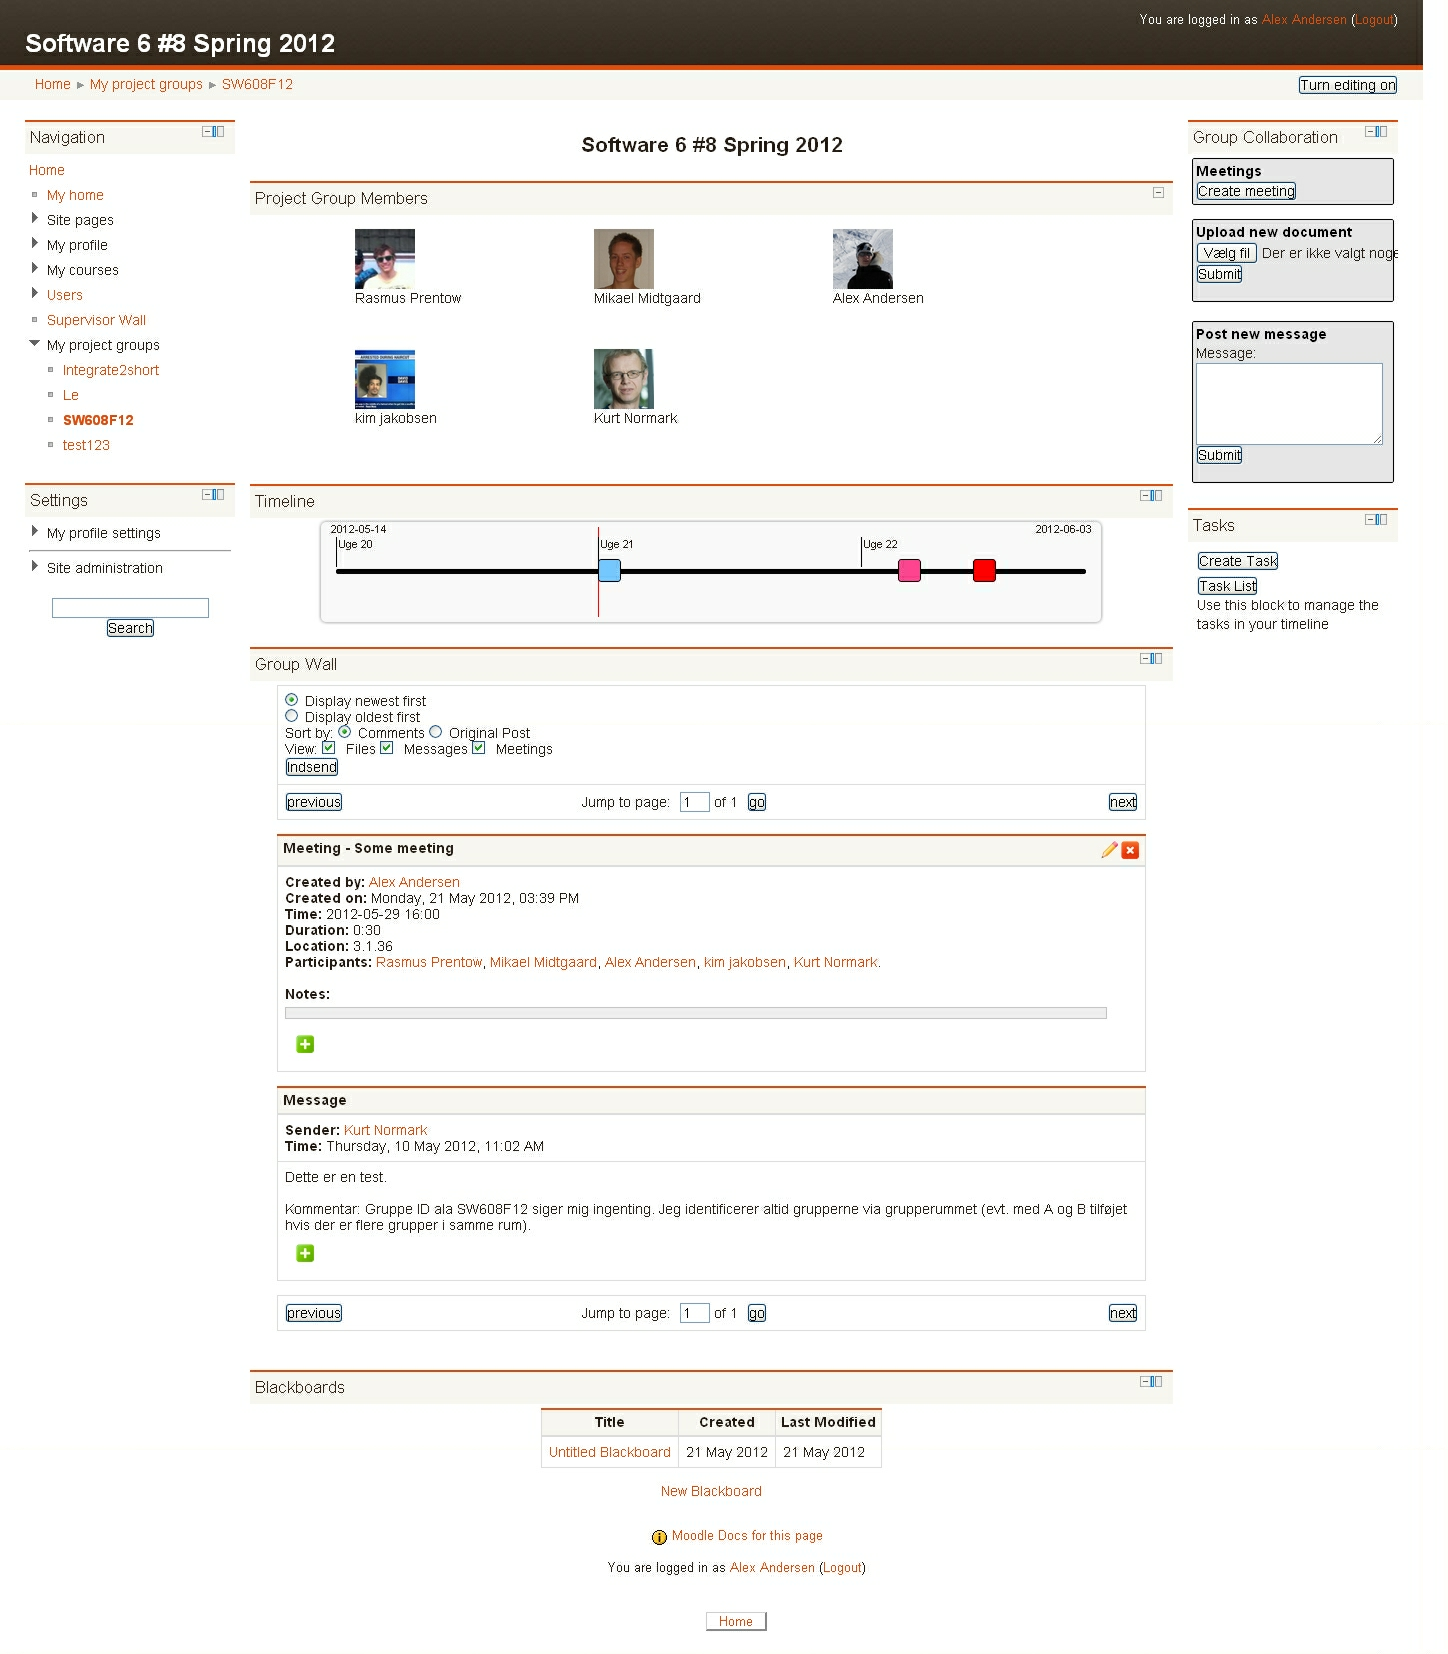
\includegraphics[width=\textwidth]{images/projectgroupnoedit.png}
	\morscaption{The project group room}
	\label{fig:projectgroupnoedit}
\end{figure}

The project group room consist of three columns. 
The left column is the standard navigation menu in Moodle. 
We do not want anything to be added to this column to ensure that the page seem familiar to the user.
The center and right columns both contain blocks.
The various blocks presented on the project groups page are described in \secref{sec:implprojectgroupblocks}. 
If a user wants to edit the block layout for the project group room he can press the ``Turn editing on'' button. 
This will add edit and move buttons to each block. 
A new block is added in editing mode to allow for adding new blocks. 
If a user edits the page, the change can be seen by all group members. 
The page in edit mode can be seen in figure \figref{fig:projectgroupwithedit}.

\begin{figure}[h]
	\centering
		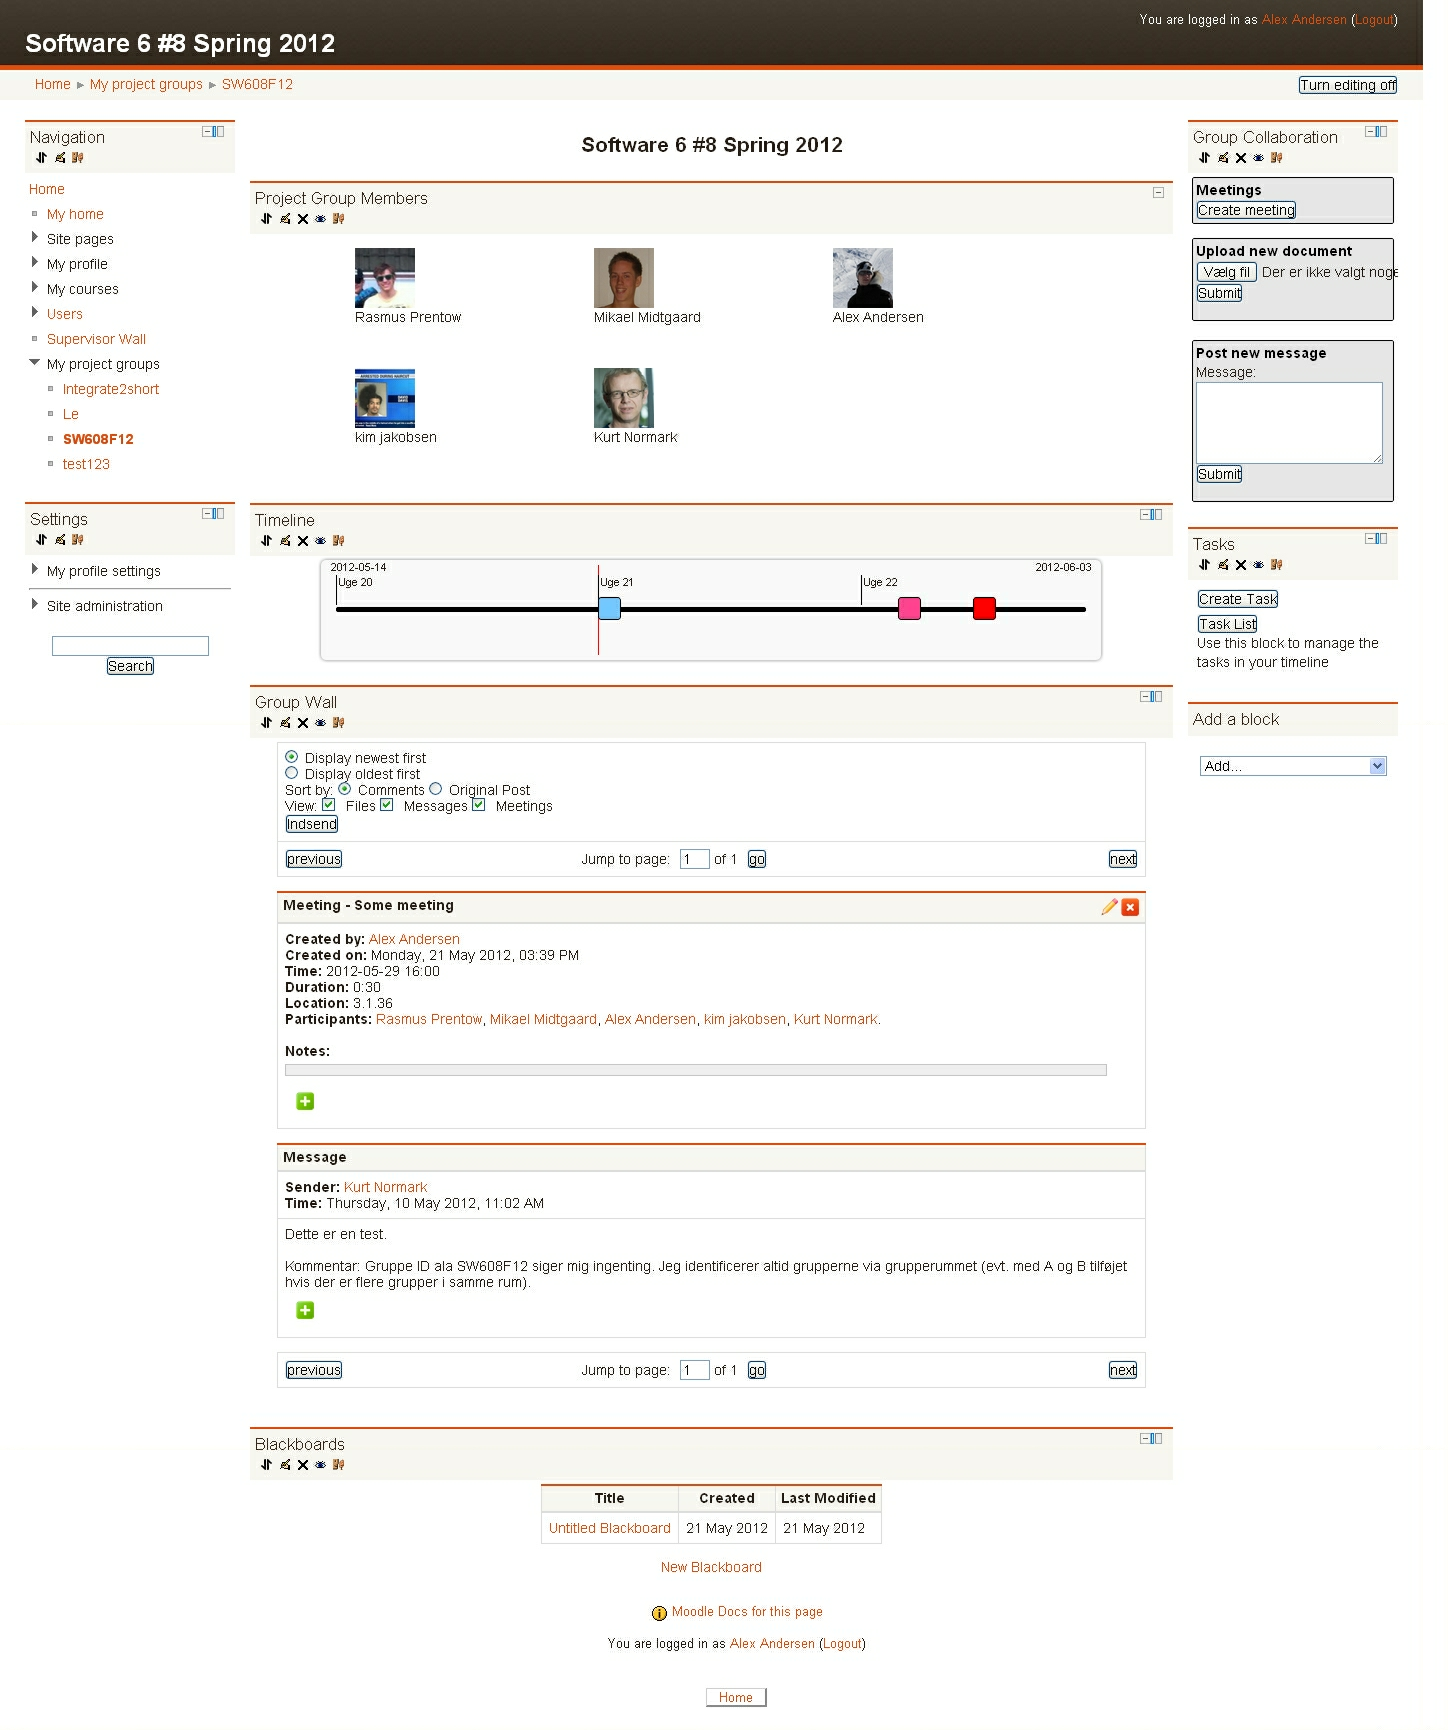
\includegraphics[width=\textwidth]{images/projectgroupwithedit.png}
	\morscaption{The project group room with editing turned on}
	\label{fig:projectgroupwithedit}
\end{figure}
